% (c) 2012 Silvia Cibola - silvia.cibola@gmail.com

% (c) 2012-2014 Dimitrios Vrettos - d.vrettos@gmail.com

\chapter{Vettori}

\section{Prime definizioni}

Sappiamo che due punti~$A$ e~$B$ presi su una retta~$a$ determinano il segmento~$b$ di estremi~$A$ e~$B$; fissiamo su di esso un verso di percorrenza, per esempio da~$A$ verso~$B$.

\begin{definizione}
Il \emph{segmento orientato} di estremi~$A$ e~$B$ si chiama \emph{vettore}; esso viene indicato con~$\overrightarrow{AB}$ oppure con~$\vec{u}$;
il punto~$A$ è il primo estremo e~$B$ il secondo estremo.
\end{definizione}

Un \emph{vettore libero} è caratterizzato da tre elementi:
\begin{itemize*}
\item la \emph{direzione} indicata dalla retta su cui esso giace;
\item il \emph{verso} indicato dalla punta della freccia che dal primo estremo va al secondo estremo;
\item il \emph{modulo} o \emph{intensità}, uguale alla misura del segmento~$AB$: scriveremo~$|\vec{u}|=\overline{AB}$ e leggeremo ``il modulo del vettore~$\vec{u}$ è
uguale alla misura del segmento~$AB$''.
\end{itemize*}

Un \emph{vettore applicato} è caratterizzato, oltre che dai tre elementi suddetti, anche dal \emph{punto di applicazione},
ovvero il punto da cui parte la freccia, chiamato anche primo estremo del vettore.

\begin{exrig}
\begin{esempio}
I due vettori~$\overrightarrow{AB}$ e~$\overrightarrow{DC}$ nella figura~\ref{fig:F.1} appartengono alla stessa retta, quindi hanno stessa direzione, verso opposto e modulo diverso.
\end{esempio}

\begin{esempio}
I due vettori~$\overrightarrow{AB}$ e~$\overrightarrow{DC}$ in figura \ref{fig:F.2} appartengono a rette parallele, quindi hanno stessa direzione. I loro versi sono opposti e hanno
uguale intensità: essi si chiamano \emph{vettori opposti} e scriveremo~$\overrightarrow{AB}=-\overrightarrow{DC}$.
\end{esempio}
\begin{esempio}
I due vettori~$\overrightarrow{AB}$ e~$\overrightarrow{CD}$ in figura \ref{fig:F.3} appartengono a rette parallele, quindi hanno stessa direzione. Hanno lo stesso verso e uguale intensità:
essi si chiamano \emph{equipollenti} e scriveremo~$\overrightarrow{AB}\equiv\overrightarrow{CD}$.
\end{esempio}
\end{exrig}

\begin{figure}[hb]
\centering
% (c) 2012 Dimitrios Vrettos - d.vrettos@gmail.com


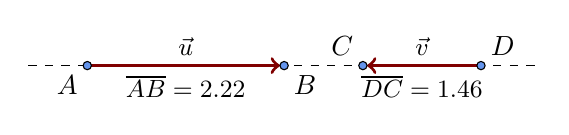
\begin{tikzpicture}[x=5mm,y=5mm]
\begin{scope}[dashed]

\draw (-1,0) -- (12,0);
\end{scope}
\begin{scope}[Maroon, very thick,->, shorten >=1.5pt]
\draw (.5,0) -- (5.5,0);
\draw  (10.5,0)--(7.5,0);
\end{scope}

\node [below left] at (.5,0) {$A$};
\node [below right] at (5.5,0) {$B$};
\node [above left] at (7.5,0) {$C$};
\node [above right] at (10.5,0) {$D$};

\begin{scope}[font=\small]
\node[below] at (9,0) {$\overline{DC}=1.46$};
\node[above] at (9,0) {$\vec{v}$};
\node[below] at (3,0) {$\overline{AB}=2.22$};
\node[above] at (3,0) {$\vec{u}$};
\end{scope}

\foreach \x in {.5,5.5,7.5,10.5}
\filldraw[fill=CornflowerBlue, draw=black] (\x,0) circle (1.5pt);
\end{tikzpicture}
\caption{I vettori hanno stessa direzione, verso opposto e modulo diverso.}\label{fig:F.1}
\end{figure}

 \begin{figure}[ht]
\begin{minipage}{0.45\textwidth}
\centering
% (c) 2012 Dimitrios Vrettos - d.vrettos@gmail.com

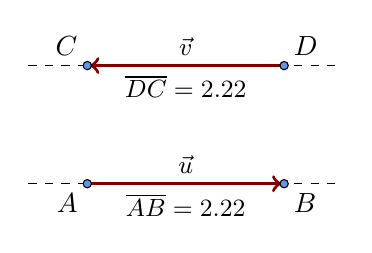
\begin{tikzpicture}[x=5mm,y=5mm]
  \begin{scope}[dashed]
    \foreach \y in {0,3}
      \draw (-1,\y) -- (7,\y);
  \end{scope}
  
  \begin{scope}[Maroon, very thick,->, shorten >=1pt]
    \draw (.5,0) -- (5.5,0);
    \draw (5.5,3) -- (.5,3) ;
  \end{scope}

  \node [below left] at (.5,0) {$A$};
  \node [below right] at (5.5,0) {$B$};
  \node [above left] at (.5,3) {$C$};
  \node [above right] at (5.5,3) {$D$};

  \begin{scope}[font=\small]
    \node[below] at (3,3) {$\overline{DC}=2.22$};
    \node[above] at (3,3) {$\vec{v}$};
    \node[below] at (3,0) {$\overline{AB}=2.22$};
    \node[above] at (3,0) {$\vec{u}$};
  \end{scope}

  \foreach \x in {.5,5.5}{
    \foreach \yi in {0,3}
      \filldraw[fill=CornflowerBlue, draw=black] (\x,\yi) circle (1.5pt);}
\end{tikzpicture}
\caption{Vettori opposti.}\label{fig:F.2}
\end{minipage}\hfil
\begin{minipage}{0.45\textwidth}
\centering
% (c) 2012 Dimitrios Vrettos - d.vrettos@gmail.com

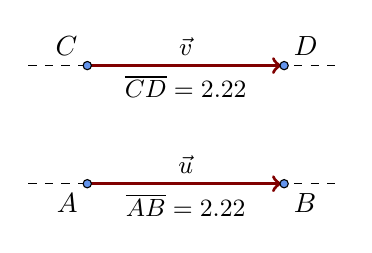
\begin{tikzpicture}[x=5mm,y=5mm]
  \begin{scope}[dashed]
    \foreach \y in {0,3}
      \draw (-1,\y) -- (7,\y);
  \end{scope}
  
  \begin{scope}[Maroon, very thick,->, shorten >=1pt]
    \draw (.5,0) -- (5.5,0);
    \draw (.5,3) -- (5.5,3);
  \end{scope}

  \node [below left] at (.5,0) {$A$};
  \node [below right] at (5.5,0) {$B$};
  \node [above left] at (.5,3) {$C$};
  \node [above right] at (5.5,3) {$D$};

  \begin{scope}[font=\small]
    \node[below] at (3,3) {$\overline{CD}=2.22$};
    \node[above] at (3,3) {$\vec{v}$};
    \node[below] at (3,0) {$\overline{AB}=2.22$};
    \node[above] at (3,0) {$\vec{u}$};
  \end{scope}

  \foreach \x in {.5,5.5}{
    \foreach \yi in {0,3}
      \filldraw[fill=CornflowerBlue, draw=black] (\x,\yi) circle (1.5pt);}
\end{tikzpicture}
\caption{Vettori equipollenti.}\label{fig:F.3}
\end{minipage}
\end{figure}

Osserviamo che un vettore può essere interpretato come uno spostamento dal primo estremo al secondo estremo, avente la direzione della retta cui appartiene il vettore stesso nel
verso indicato dalla freccia.
Nel piano dotato di riferimento cartesiano ortogonale (figura~\ref{fig:F.4} (a)) è rappresentato il vettore~$\vec{u}=\overrightarrow{AB}$ avente il primo estremo nel punto~$A(-2;1)$ e
il secondo estremo
in~$B(1;2)$. Per andare da~$A$ a~$B$ si possono compiere diversi percorsi: possiamo procedere sul vettore~$\vec{u}$ oppure possiamo scegliere di compiere due spostamenti particolari,
uno parallelo all'asse~$x$ e l'altro parallelo all'asse~$y$. In tal modo si determina il punto~$C(1;1)$ come ``tappa intermedia'' per raggiungere~$B$:
ci spostiamo sul vettore~$\overrightarrow{AC}$ e poi da~$C$ sul vettore~$\overrightarrow{CB}$.

\begin{figure}[htb]
\centering
% (c) 2012 Dimitrios Vrettos - d.vrettos@gmail.com

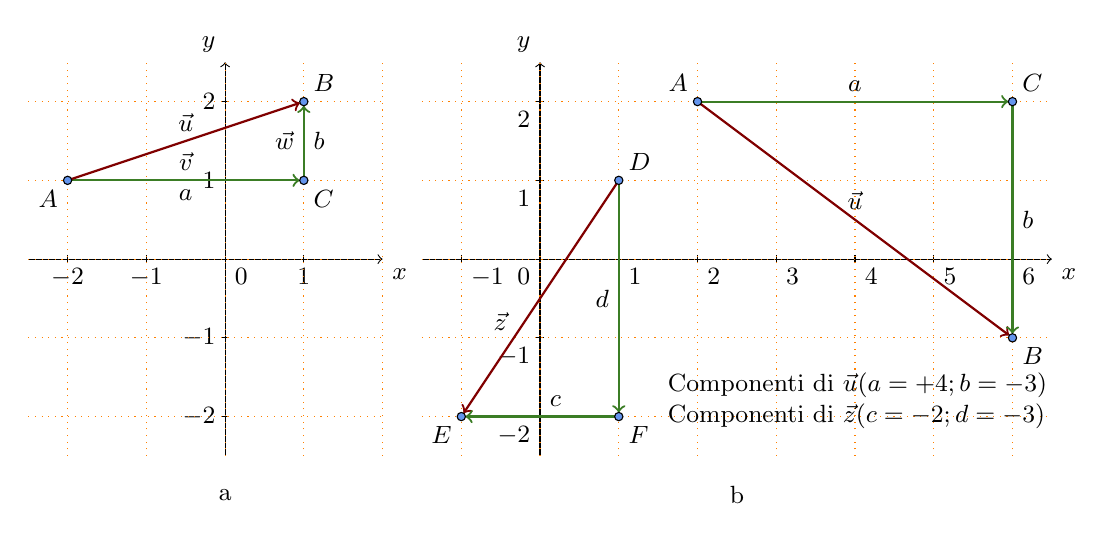
\begin{tikzpicture}[x=10mm,y=10mm, font=\small]

  \begin{scope}[->]
    \draw (-2.5,0) -- (2,0) node [below right] () {$x$};
    \draw (0,-2.5) -- (0,2.5) node[above left] {$y$};
  \end{scope}

  \foreach \x/\xtext in {-2/-2,-1/-1, 1/1}{
    \node[below] at (\x,0) {$\xtext$};
    \draw (\x,1.5pt) -- (\x,-1.5pt);}
  \foreach \y/\ytext in {-2/-2,-1/-1, 1/1, 2/2}{
    \node[left] at (0,\y) {$\ytext$};
    \draw (1.5pt,\y) -- (-1.5pt,\y);}
  \node[below right] at (0,0) {$0$};

  \node[below left] at (-2,1) {$A$};
  \node[above right] at (1,2) {$B$};
  \node[below right] at (1,1) {$C$};

  \node[above] at (-.5,1.5) {$\vec{u}$};
  
  \node[above] at (-.5,1) {$\vec{v}$};
  \node[below] at (-.5,1) {$a$};
  \node[left] at (1,1.5) {$\vec{w}$};
  \node[right] at (1,1.5) {$b$};

\node at (0,-3) {a};
  \begin{scope}[dotted, orange]
    \draw (-2.5,-2.5) grid (2,2.5);
  \end{scope}

  \begin{scope}[thick, OliveGreen, shorten >=1.5pt, ->]
    \draw (-2,1) -- (1,1);
    \draw[Maroon] (-2,1) -- (1,2);
    \draw (1,1) -- (1,2);
  \end{scope}
  
  \begin{scope}[fill=CornflowerBlue, draw=black]
    \filldraw (-2,1) circle (1.5pt);
    \filldraw (1,2) circle (1.5pt);
    \filldraw (1,1) circle (1.5pt);
  \end{scope}

  \begin{scope}[xshift=40mm]
    \begin{scope}[->]
    \draw (-1.5,0) -- (6.5,0) node [below right] () {$x$};
    \draw (0,-2.5) -- (0,2.5) node[above left] {$y$};
    \end{scope}

    \foreach \x/\xtext in {-1/-1, 1/1,2/2,3/3,4/4,5/5,6/6}{
      \node[below right] at (\x,0) {$\xtext$};
      \draw (\x,1.5pt) -- (\x,-1.5pt);}
    \foreach \y/\ytext in {-2/-2,-1/-1, 1/1, 2/2}{
      \node[below left] at (0,\y) {$\ytext$};
      \draw (1.5pt,\y) -- (-1.5pt,\y);}
    \node[below left] at (0,0) {$0$};

    \node[above left] at (2,2) {$A$};
    \node[below right] at (6,-1) {$B$};
    \node[above right] at (6,2) {$C$};

    \node[above] at (4,2) {$a$};
    \node[right] at (6,.5) {$b$};
    \node[above] at (4,.5) {$\vec{u}$};

    \node[above right] at (0,-2) {$c$};
    \node[left] at (1,-.5) {$d$};
    \node[left] at (-.3,-.8) {$\vec{z}$};

    \node[above right] at (1,1) {$D$};
    \node[below right] at (1,-2) {$F$};
    \node[below left] at (-1,-2) {$E$};

    \node at (2.5,-3) {b};
    \begin{scope}[dotted, orange]
      \draw (-1.5,-2.5) grid (6.5,2.5);
    \end{scope}

    \begin{scope}[thick, shorten >=1.5pt, ->]
      \begin{scope}[Maroon]
	\draw(2,2) -- (6,-1);
	\draw (1,1) -- (-1,-2);
      \end{scope}
      
      \begin{scope}[OliveGreen]
	\draw(2,2) -- (6,2);
	\draw (6,2) -- (6,-1);

	\draw (1,1) -- (1,-2);
	\draw (1,-2) -- (-1,-2);
	\end{scope}
    \end{scope}

    \begin{scope}[fill=CornflowerBlue, draw=black]
      \filldraw (6,2) circle (1.5pt);
      \filldraw (2,2) circle (1.5pt);
      \filldraw (6,-1) circle (1.5pt);

      \filldraw (1,1) circle (1.5pt);
      \filldraw (1,-2) circle (1.5pt);
      \filldraw (-1,-2) circle (1.5pt);
    \end{scope}

    \node[right] () at (1.5,-1.6) {Componenti di $\vec{u}(a=+4;b=-3)$};
    \node[right] () at (1.5,-2) {Componenti di $\vec{z}(c=-2;d=-3)$};
  \end{scope}
\end{tikzpicture}
\caption{Spostamenti di vettori.}\label{fig:F.4}
\end{figure}

\begin{definizione}
Chiamiamo \emph{componenti} del vettore~$\overrightarrow{AB}$ le \emph{misure con segno} dei segmenti~$AC$ e~$CB$ paralleli a quelli degli assi coordinati, con la precisazione di assegnare il segno~$+$ alle misure
dello spostamento avente lo stesso verso degli assi coordinati e segno~$-$ se il verso è opposto a quello degli assi coordinati.
\end{definizione}

In figura \ref{fig:F.4} (a) le componenti del vettore assegnato sono positive in quanto sia lo spostamento orizzontale che quello verticale avvengono nello stesso
verso degli assi coordinati. Scriveremo~$\overrightarrow{AB}(+3;+1)$. Tutti i vettori del piano cartesiano di componenti~$(+3;+1)$ sono equipollenti a~$\overrightarrow{AB}$.
Ciò che li distingue in modo univoco è il loro punto di applicazione.

\begin{exrig}
\begin{esempio}
Il vettore~$\vec{z}$ della figura \ref{fig:F.4} (b) ha componenti entrambe negative poiché lo spostamento orizzontale e quello verticale avvengono in verso
contrario rispetto al verso degli assi coordinati: scriveremo~$\vec{z}(-2;-3)$. Il vettore~$\vec{u}$ della figura \ref{fig:F.4} (b) ha la componente
lungo l'asse~$x$ positiva e quella verticale negativa: scriveremo~$\vec{u}(+4;-3)$.
\end{esempio}
\end{exrig}

\begin{procedura}
Determinare le componenti cartesiane di un vettore~$\vec{v}$, note le coordinate cartesiane degli estremi~$A(x_A;y_A)$ e~$B(x_B;y_B)$:
\begin{enumeratea}
\item dal primo estremo tracciamo la parallela all'asse~$x$ e dal secondo estremo la parallela all'asse~$y$ determinando il punto~$C(x_B;y_A)$;
\item calcoliamo le misure con segno~$a=x_B-x_A$, $b=y_B-y_A$;
\item scriviamo~$\vec{v}(a;b)$ ovvero~$\vec{v}(x_B-x_A;b=y_B-y_A)$.
\end{enumeratea}
\end{procedura}

Ottenute le componenti si determina il \emph{modulo del vettore} utilizzando il teorema di Pitagora; si ha infatti~$|\vec{u}|=\overline{AB}=\sqrt{a^2+b^2}=\sqrt{(x_B-x_A)^2+(y_B-y_A)^2}$.
Il rapporto~$m_{\vec{u}}=\dfrac{b}{a}=\dfrac{y_B-y_A}{x_B-x_A}$ indica invece la \emph{direzione del vettore}.
	
\begin{exrig}
\begin{esempio}
\begin{multicols}{2}
Assegnato il vettore della figura a fianco, determinate le sue componenti, il modulo e la direzione. Completate i passi indicati nella strategia risolutiva:
 \begin{itemize*}
\item scrivete le coordinate degli estremi del vettore assegnato~$A(\ldots;\ldots)$ e~$B(\ldots;\ldots)$;
\item individuate le componenti del vettore~$\vec{w}$:
\begin{itemize*}
\item segnate il punto~$C(\ldots;\ldots)$ e calcolate $a=x_B-x_A$ e~$b=y_B-y_A$;
\item le componteni del vettore sono $\vec{w}(\ldots;\ldots)$;
\end{itemize*}
\item determinate il modulo del vettore~$|\vec{w}|=\sqrt{\vphantom{0}\ldots\ldots}$;
\item determinate la direzione del vettore~$m_{\vec{w}}=\ldots$.
\end{itemize*}
\begin{center}
 % (c) 2012 Dimitrios Vrettos - d.vrettos@gmail.com

\begin{tikzpicture}[x=10mm,y=10mm, font=\small]

  \begin{scope}[->]
   \draw (-2,0) -- (3,0) node[below right] {$x$};
    \draw (0,-3) -- (0,3) node[above left] {$y$};
  \end{scope}

  \foreach \x/\xtext in {-1/-1, 1/1,2/2}{
    \node[below] at (\x,0) {$\xtext$};
    \draw (\x,1.5pt) -- (\x,-1.5pt);}
  \foreach \y/\ytext in {-2/-2,-1/-1, 1/1, 2/2}{
    \node[left] at (0,\y) {$\ytext$};
    \draw (1.5pt,\y) -- (-1.5pt,\y);}
  \node[below right] at (0,0) {$0$};

  \begin{scope}[dotted, orange]
    \draw (-2,-3) grid (3,3);
  \end{scope}

  \begin{scope}[thick, Maroon, shorten >=1.5pt, ->]
    \draw (-1,-2) -- (2,2);
      \end{scope}
  
\begin{scope}[fill=CornflowerBlue, draw=black]
\filldraw (2,2) circle (1.5pt) node[above right] {$B$};
\filldraw (-1,-2) circle (1.5pt) node[below left] {$A$};
\end{scope}

\node at (.5,.5) {$\vec{w}$};

\end{tikzpicture}

\end{center}
\end{multicols}
\end{esempio}

\begin{esempio}
\begin{multicols}{2}
 Tracciate nel riferimento cartesiano ortogonale il vettore~$\vec{v}(1;-3)$. Nella richiesta di questo quesito sembra manchi qualcosa: conosciamo
le componenti del vettore, ma dove mettiamo il primo estremo? Provate a mettere il primo estremo in ciascuno dei seguenti punti:~$A_1(-1;2)$, $A_2(1;0)$, $A_3(3;-2)$
e determinate il secondo estremo di ciascun vettore; completate indicando per ciascuno di essi il modulo e la direzione. È vero che tutti i vettori tracciati sono equipollenti?
In figura è rappresentato il vettore equipollente a quelli costruiti avente il primo estremo nell'origine del riferimento?
\begin{center}
 % (c) 2012 Dimitrios Vrettos - d.vrettos@gmail.com

\begin{tikzpicture}[x=10mm,y=10mm, font=\small]

  \begin{scope}[->]
    \draw (-1.5,0) -- (2.5,0) node [below right] () {$x$};
    \draw (0,-3.5) -- (0,1.5) node[above left] {$y$};
  \end{scope}

  \foreach \x/\xtext in {-1/-1, 1/1,2/2}{
    \node[below] at (\x,0) {$\xtext$};
    \draw (\x,1.5pt) -- (\x,-1.5pt);}
  \foreach \y/\ytext in {-3/-3,-2/-2,-1/-1, 1/1}{
    \node[left] at (0,\y) {$\ytext$};
    \draw (1.5pt,\y) -- (-1.5pt,\y);}
  \node[below left] at (0,0) {$0$};

  \begin{scope}[dotted, orange]
    \draw (-1.5,-3.5) grid (2.5,1.5);
  \end{scope}

  \begin{scope}[thick, Maroon, shorten >=1.5pt, ->]
    \draw (-0,0) -- (1,-2);
      \end{scope}
  
\begin{scope}[fill=CornflowerBlue, draw=black]
\filldraw (1,-2) circle (1.5pt) node[below right] {$B$};
\filldraw (0,0) circle (1.5pt) node[above left] {$A$};
\end{scope}

\node at (.8,-1) {$\vec{u}$};

\end{tikzpicture}
\end{center}

\end{multicols}

\osservazione
Quando si assegna un vettore (libero) mediante le sue componenti, collocheremo il primo estremo
nell'origine del riferimento cartesiano ortogonale e il secondo estremo (punta della freccia) avrà come
coordinate le componenti del vettore in questione.
\end{esempio}
\end{exrig}

\ovalbox{\risolvi \ref{ese:B.1}}

\section{Operazioni con i vettori}

\subsection{Somma di vettori}

\begin{definizione}
Nel punto~$A$ del piano sono applicati due vettori~$\vec{u}$ e~$\vec{v}$: dall'estremo~$B$ si
traccia la retta parallela ad~$AC$ e da~$C$ la parallela ad~$AB$ indicando con~$D$ il loro punto di intersezione.
Si definisce \emph{somma dei vettori}~$\vec{u}$ e~$\vec{v}$ il vettore~$\vec{w}$ individuato dalla diagonale~$AD$ del parallelogramma $ABDC$ e si scrive~$\vec{w}=\vec{u}+\vec{v}$.
\end{definizione}

\begin{figure}[h]
\centering
% (c) 2012 Dimitrios Vrettos - d.vrettos@gmail.com

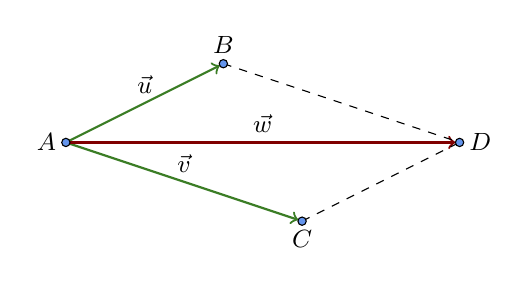
\begin{tikzpicture}[x=10mm,y=10mm, font=\small]

  \begin{scope}[thick,shorten >=1.5pt, ->]
    \begin{scope}[OliveGreen]
      \draw (0,0) -- (2,1);
      \draw (0,0) -- (3,-1);
    \end{scope}  
    
    \begin{scope}[Maroon]
      \draw (0,0) -- (5,0);
    \end{scope}
  \end{scope}

  \begin{scope}[dashed]
    \draw[xshift=30mm,yshift=-10mm] (0,0) -- (2,1);
    \draw[xshift=20mm,yshift=10mm] (0,0) -- (3,-1);
  \end{scope}

  \begin{scope}[fill=CornflowerBlue, draw=black]
    \filldraw (5,0) circle (1.5pt) node[right] {$D$};
    \filldraw (0,0) circle (1.5pt) node[left] {$A$};
    \filldraw (2,1) circle (1.5pt) node[above] {$B$};
    \filldraw (3,-1) circle (1.5pt) node[below] {$C$};
  \end{scope}

  \node[above] at (1,0.5) {$\vec{u}$};
  \node[above] at (1.5,-0.5) {$\vec{v}$};
  \node[above] at (2.5,0) {$\vec{w}$};

\end{tikzpicture}
 \caption{Somma di due vettori.}\label{fig:F.5}
\end{figure}

Nella sua opera ``Philosophiae naturalis principia mathematica'' del~1682, Isaac Newton\footnote{matematico, fisico, filosofo, astronomo, teologo e alchimista inglese (1642 - 1727).} nel primo corollario alle leggi del moto,
scrive: <<un corpo spinto da due forze congiunte descriverà la diagonale di un parallelogramma nello stesso tempo nel quale descriverebbe separatamente i lati>>.

\vspazio\ovalbox{\risolvi \ref{ese:B.2}}

Illustriamo con un esempio che per la somma di vettori vale la proprietà associativa.

\begin{exrig}
\begin{esempio}
Dimostriamo che vale~$\vec{u}+(\vec{v}+\vec{w})=(\vec{u}+\vec{v})+\vec{w}$.

Nella figura \ref{fig:F.6} è realizzata la costruzione~$\vec{v}+\vec{w}=\vec{k}$ e~$\vec{u}+\vec{k}=\vec{j}$.
Nella figura \ref{fig:F.7} è realizzata la costruzione~$\vec{u}+\vec{v}=\vec{z}$ e~$\vec{z}+\vec{w}=\vec{j}$.
Sovrapponendo le due figure si può constatare che i due vettori~$\vec{j}$ risultanti coincidono.
\end{esempio}
\end{exrig}

\begin{figure}[t]
\begin{minipage}{.45\textwidth}
 \centering
 % (c) 2012 Dimitrios Vrettos - d.vrettos@gmail.com

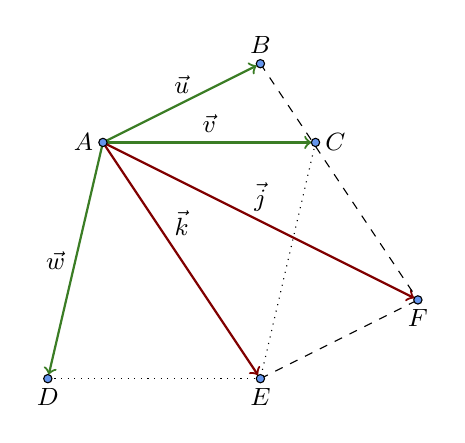
\begin{tikzpicture}[x=10mm,y=10mm, font=\small]

  \begin{scope}[thick,shorten >=1.5pt, ->]
    \begin{scope}[OliveGreen]
      \draw (0,0) -- (2,1); % vettore u
      \draw (0,0) -- (2.7,0); % vettore v
      \draw (0,0) -- (-.7,-3); % vettore w
    \end{scope}  
    
    \begin{scope}[Maroon]
      \draw (0,0) -- (4,-2); % vettore j
      \draw (0,0) -- (2,-3); % vettore k    
    \end{scope}
  \end{scope}

  \begin{scope}[dashed]
    \draw[xshift=20mm,yshift=-30mm] (0,0) -- (2,1);
    \draw[xshift=20mm,yshift=10mm] (0,0) -- (2,-3);
  \end{scope}

  \begin{scope}[dotted]
    \draw[xshift=-7mm,yshift=-30mm] (0,0) -- (2.7,0);
    \draw[xshift=27mm,yshift=0mm] (0,0) -- (-.7,-3);
  \end{scope}  

  \begin{scope}[fill=CornflowerBlue, draw=black]
    \filldraw (0,0) circle (1.5pt) node[left] {$A$};
    \filldraw (2,1) circle (1.5pt) node[above] {$B$};
    \filldraw (2,-3) circle (1.5pt) node[below] {$E$};
    \filldraw (4,-2) circle (1.5pt) node[below] {$F$};
    \filldraw (-.7,-3) circle (1.5pt) node[below] {$D$};
    \filldraw (2.7,0) circle (1.5pt) node[right] {$C$};
  \end{scope}

  \node[above] at (1,.5) {$\vec{u}$};
  \node[above] at (1.35,0) {$\vec{v}$};
  \node[above] at (2,-1) {$\vec{j}$};
  \node[above] at (1,-1.3) {$\vec{k}$};
  \node at (-.6,-1.5) {$\vec{w}$};

\end{tikzpicture}
 \caption{$\vec{v}+\vec{w}=\vec{k}$ e~$\vec{u}+\vec{k}=\vec{j}$.}
 \label{fig:F.6}
\end{minipage}\hfil
\begin{minipage}{.45\textwidth}
 \centering
 % (c) 2012 Dimitrios Vrettos - d.vrettos@gmail.com

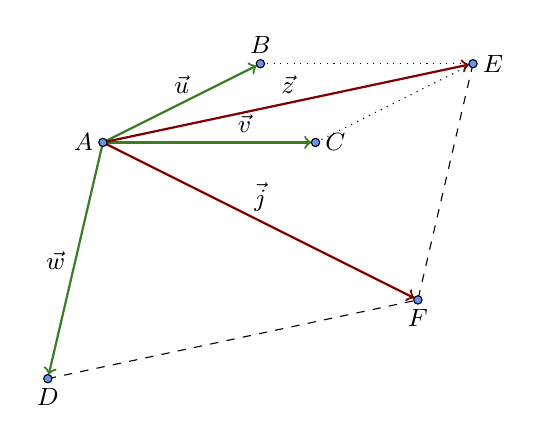
\begin{tikzpicture}[x=10mm,y=10mm, font=\small]

  \begin{scope}[thick,shorten >=1.5pt, ->]
    \begin{scope}[OliveGreen]
      \draw (0,0) -- (2,1); % vettore u
      \draw (0,0) -- (2.7,0); % vettore v
      \draw (0,0) -- (-.7,-3); % vettore w
    \end{scope}
    
    \begin{scope}[Maroon]
      \draw (0,0) -- (4,-2); % vettore j
      \draw (0,0) -- (4.7,1); % vettore z    
    \end{scope}
  \end{scope}

  \begin{scope}[dashed]
    \draw[xshift=47mm,yshift=10mm] (0,0) -- (-.7,-3);
    \draw[xshift=-7mm,yshift=-30mm] (0,0) -- (4.7,1);
  \end{scope}

  \begin{scope}[dotted]
    \draw[xshift=20mm,yshift=10mm] (0,0) -- (2.7,0);
    \draw[xshift=27mm,yshift=0mm] (0,0) -- (2,1);
  \end{scope}  

  \begin{scope}[fill=CornflowerBlue, draw=black]
    \filldraw (0,0) circle (1.5pt) node[left] {$A$};
    \filldraw (2,1) circle (1.5pt) node[above] {$B$};
    \filldraw (4.7,1) circle (1.5pt) node[right] {$E$};
    \filldraw (4,-2) circle (1.5pt) node[below] {$F$};
    \filldraw (-.7,-3) circle (1.5pt) node[below] {$D$};
    \filldraw (2.7,0) circle (1.5pt) node[right] {$C$};
  \end{scope}

  \node[above] at (1,.5) {$\vec{u}$};
  \node[above] at (1.8,0) {$\vec{v}$};
  \node[above] at (2,-1) {$\vec{j}$};
  \node[above] at (2.35,.5) {$\vec{z}$};
  \node at (-.6,-1.5) {$\vec{w}$};

\end{tikzpicture}
 \caption{$\vec{u}+\vec{v}=\vec{z}$ e~$\vec{z}+\vec{w}=\vec{j}$.}
 \label{fig:F.7}
\end{minipage}
\end{figure}

Osserviamo che la validità della proprietà associativa ci permette di costruire la somma di più vettori. Per come è definita l'operazione di somma, pensando al
vettore come rappresentante di uno spostamento dal primo estremo al secondo, possiamo interpretare la figura \ref{fig:F.5} come lo spostamento di un punto prima
da~$A$ fino a~$B$ e poi da questo fino a~$D$, essendo~$\overrightarrow{BD}$ un vettore equipollente ad~$\overrightarrow{AC}$ (cambia soltanto il punto di applicazione). Quindi possiamo affermare che il vettore somma
di due vettori~$\vec{u}$ e~$\vec{v}$ si può determinare prendendo due vettori~$\overrightarrow{AB}$ e~$\overrightarrow{BC}$ rispettivamente equipollenti
ai dati; se~$\overrightarrow{AB} \equiv \vec{u}$ e~$\overrightarrow{BC} \equiv \vec{v}$ allora la somma è il vettore~$\overrightarrow{AC}$ avente~$A$
come primo estremo e~$C$
come secondo estremo (figura \ref{fig:F.8}).

Pertanto la somma di più vettori si può semplicemente determinare scegliendo per ogni addendo il vettore equipollente avente il primo estremo nell'estremo finale
dell'addendo precedente: la somma è il vettore avente il primo estremo nel punto iniziale del primo addendo e l'estremo finale nel secondo estremo dell'ultimo addendo.
\begin{exrig}
\begin{esempio}
Somma di più vettori:~$\vec{z}+\vec{a}+\vec{b}+\vec{c}=\vec{s}$~~(figura \ref{fig:F.9}).
\end{esempio}
\end{exrig}

\begin{figure}[hb]
\begin{minipage}[t]{.45\textwidth}
 \centering
 % (c) 2012 Dimitrios Vrettos - d.vrettos@gmail.com

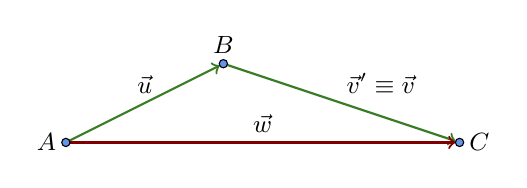
\begin{tikzpicture}[x=10mm,y=10mm, font=\small]

  \begin{scope}[thick,shorten >=1.5pt, ->]
    \begin{scope}[OliveGreen]
      \draw (0,0) -- (2,1);
      \draw (2,1) -- (5,0);
    \end{scope}  
    
    \begin{scope}[Maroon]
      \draw (0,0) -- (5,0);
    \end{scope}
  \end{scope}


  \begin{scope}[fill=CornflowerBlue, draw=black]
    \filldraw (5,0) circle (1.5pt) node[right] {$C$};
    \filldraw (0,0) circle (1.5pt) node[left] {$A$};
    \filldraw (2,1) circle (1.5pt) node[above] {$B$};
  \end{scope}

  \node[above] at (1,0.5) {$\vec{u}$};
  \node[above] at (4,0.5) {$\vec{v}' \equiv \vec{v}$};
  \node[above] at (2.5,0) {$\vec{w}$};

\end{tikzpicture}
 \caption{Somma di due vettori.}
 \label{fig:F.8}
\end{minipage}\hfil
\begin{minipage}[t]{.45\textwidth}
 \centering
 % (c) 2012 Dimitrios Vrettos - d.vrettos@gmail.com

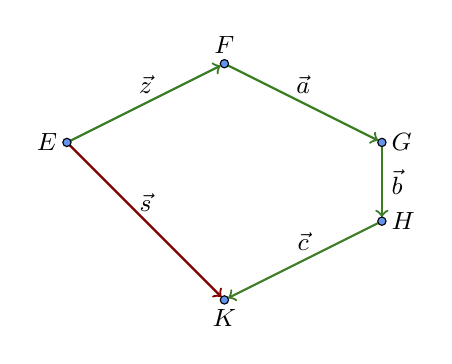
\begin{tikzpicture}[x=10mm,y=10mm, font=\small]

  \begin{scope}[thick,shorten >=1.5pt, ->]
    \begin{scope}[OliveGreen]
\draw (-2,2) -- (0,3);
\draw (0,3) -- (2,2);
\draw (2,2) -- (2,1);
\draw (2,1) -- (0,0);
    \end{scope}  
    
    \begin{scope}[Maroon]
      \draw (-2,2) -- (0,0);
    \end{scope}
  \end{scope}


  \begin{scope}[fill=CornflowerBlue, draw=black]
    \filldraw (-2,2) circle (1.5pt) node[left] {$E$};
    \filldraw (0,3) circle (1.5pt) node[above] {$F$};
    \filldraw (2,2) circle (1.5pt) node[right] {$G$};
    \filldraw (2,1) circle (1.5pt) node[right] {$H$};
    \filldraw (0,0) circle (1.5pt) node[below] {$K$};
  \end{scope}

  \node[above] at (-1,2.5) {$\vec{z}$};
  \node[above] at (1,2.5) {$\vec{a}$};
  \node[right] at (2,1.5) {$\vec{b}$};
  \node[above] at (1,.5) {$\vec{c}$};
  \node[above] at (-1,1) {$\vec{s}$};

\end{tikzpicture}
 \caption{Somma di più vettori.}
 \label{fig:F.9}
\end{minipage}
\end{figure}

Abbiamo visto come si costruisce geometricamente il vettore somma di vettori; vediamo come si determinano le componenti del vettore somma se la questione
è posta nel riferimento cartesiano ortogonale.

\begin{exrig}
\begin{esempio}
Nel piano dotato di riferimento cartesiano ortogonale costruiamo il vettore somma dei vettori~$\vec{u}(1;2)$ e~$\vec{v}(3;-1)$ e determiniamone
le componenti (figura~\ref{fig:F.10}).

Strategia risolutiva:
\begin{enumeratea}
\item posizioniamo i vettori~$\vec{u}$ e~$\vec{v}$ con il punto di applicazione nell'origine del sistema cartesiano;
\item costruiamo il vettore~$\vec{w}$ equipollente al vettore~$\vec{v}$ applicato al punto~$A$;
\item determiniamo il punto	$D(4;1)$;
\item costruiamo il vettore~$\vec{z}=\vec{u}+\vec{v}$ di coordinate~$\vec{z}(4;1)$.
\end{enumeratea}
Osserviamo che il primo passo realizzato ci permette di affermare~$x_z=x_u+x_v$ e~$y_z=y_u+y_v$.
\end{esempio}
\end{exrig}
%\newpage
\begin{figure}[t]
\centering
% (c) 2012 Dimitrios Vrettos - d.vrettos@gmail.com

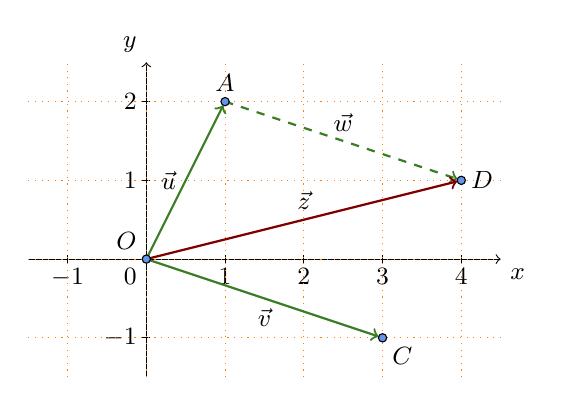
\begin{tikzpicture}[x=10mm,y=10mm, font=\small]

  \begin{scope}[->]
    \draw (-1.5,0) -- (4.5,0) node [below right] () {$x$};
    \draw (0,-1.5) -- (0,2.5) node[above left] {$y$};
  \end{scope}

  \foreach \x/\xtext in {-1/-1, 1/1,2/2,3/3,4/4}{
    \node[below] at (\x,0) {$\xtext$};
    \draw (\x,1.5pt) -- (\x,-1.5pt);}
  \foreach \y/\ytext in {-1/-1, 1/1,2/2}{
    \node[left] at (0,\y) {$\ytext$};
    \draw (1.5pt,\y) -- (-1.5pt,\y);}
  \node[below left] at (0,0) {$0$};

  \begin{scope}[dotted, orange]
    \draw (-1.5,-1.5) grid (4.5,2.5);
  \end{scope}

  \begin{scope}[thick, shorten >=1.5pt, ->]
  
	\draw[OliveGreen] (0,0) -- (1,2);
	\draw[OliveGreen] (0,0) -- (3,-1);
	\draw[OliveGreen, dashed] (1,2) -- (4,1);  
	\draw[Maroon] (-0,0) -- (4,1);
      \end{scope}
  
\begin{scope}[fill=CornflowerBlue, draw=black]
\filldraw (1,2) circle (1.5pt) node[above] {$A$};
\filldraw (0,0) circle (1.5pt) node[above left] {$O$};
\filldraw (4,1) circle (1.5pt) node[right] {$D$};
\filldraw (3,-1) circle (1.5pt) node[below right] {$C$};
\end{scope}

\node[left] at (.5,1) {$\vec{u}$};
\node[above] at (2.5,1.5) {$\vec{w}$};
\node[above] at (2,.5) {$\vec{z}$};
\node[below] at (1.5,-.5) {$\vec{v}$};
\end{tikzpicture}
\caption{Determinazione delle componenti di un vettore.}\label{fig:F.10}
\end{figure}

\begin{procedura} Note le componenti cartesiane dei vettori addendi~$\vec{u}=(x_u;y_u)$ e~$\vec{v}=(x_v;y_v)$ le
 componenti cartesiane del vettore somma~$\vec{z}=(x_z;y_z)$ si ottengono con la regola del parallelogramma:

Il primo passo realizzato nella costruzione precedente ci permette di affermare che le componenti del vettore somma $\vec{z}$ sono la somma
delle componenti dei vettori addendi:\[x_z=x_u+x_v\quad\text{e}\quad y_z=y_u+y_v.\]
\end{procedura}

\ovalbox{\risolvi \ref{ese:B.3}}

\paragraph{Applicazioni dei vettori}
I vettori sono degli enti geometrici che vengono spesso utilizzati in fisica per rappresentare tutte le grandezze che sono definite conoscendo modulo, direzione,
verso e punto di applicazione. Esempi di grandezze vettoriali sono: la velocità, l'accelerazione, la forza, il campo elettrico.

\begin{exrig}
\begin{esempio}
Nella figura seguente sono rappresentate tre scatole viste dall'alto e su ognuna di esse agiscono due forze, come rappresentato in figura. Calcola la forza risultante $\vec{r}$ in ognuno dei casi,
sapendo che una forza ha modulo~$4 \unit{N}$ e l'altra~$9 \unit{N}$.
\begin{center}
 % (c) 2012 Dimitrios Vrettos - d.vrettos@gmail.com
\begin{tikzpicture}[ x=7.5mm, y=7.5mm, font=\small]
\begin{scope}[->]
\draw (0,0) -- (0,3.5) node[left] {$y$};
\draw (0,0) -- (3.5,0) node[below] {$x$};
\end{scope}

\begin{scope}[Maroon, dotted, step=7.5mm]
\draw (0,0) grid (3.5,3.5);
\end{scope}

\foreach \x/\xtext in {1/1,2/2,3/3}{
\node[below] at (\x,0) {\xtext};
\node[left] at (0,\x) {\xtext};
}
\foreach \x in {1,2,3}{
\draw (\x,1.5pt) -- (\x,-1.5pt);
\draw (1.5pt,\x) -- (-1.5pt,\x);}
\node[below left] at (0,0) {0};
\begin{scope}[very thick, draw=CornflowerBlue, decoration={crosses, shape size=1.5mm}]
\draw decorate {(1,1) -- (1,1.1)};
\draw decorate {(2,2) -- (2,2.1)};
\draw decorate {(1,3) -- (1,3.1)};
\draw decorate {(2,1) -- (2,1.1)};
\draw decorate {(3,2) -- (3,2.1)};
\draw decorate {(3,3) -- (3,3.1)};
\end{scope}
\end{tikzpicture}
\end{center}
\newpage
\emph{Svolgimento:}
\begin{enumeratea}
\item Nel primo caso ($A$) i due vettori hanno la stessa direzione e lo stesso verso, quindi la risultante si ottiene addizionando semplicemente i due moduli:~$|\vec{r}|=4 +9 =13 \unit{N}$;
\item Nel secondo caso ($B$) poiché i vettori sono opposti come verso, si procede sottraendo al vettore maggiore il vettore minore e la forza risultante ha la direzione ed il verso
del vettore di modulo maggiore:~$|\vec{r}|=9 - 5 =4 \unit{N}$.
\item Nel terzo caso ($C$) i due vettori hanno direzioni perpendicolari, quindi il vettore somma si ottiene con il metodo del parallelogramma. Il suo modulo si ottiene applicando il teorema di Pitagora:
\[|\vec{r}|=\sqrt{4^2+9^2}=\sqrt{97}\simeq \np[N]{9,85}.\]
\end{enumeratea}
\end{esempio}
\end{exrig}

\subsection{Differenza tra vettori}

\begin{procedura} Per determinare la \emph{differenza tra due vettori} (figura~\ref{fig:F.11}) $\vec{u}$ e~$\vec{v}$
si procede nel seguente modo:
\begin{enumeratea}
\item costruiamo il vettore~$\vec{z}=-\vec{v}$ che ha stessa direzione, stesso modulo, ma verso opposto;
\item determiniamo con la regola del parallelogramma~$\vec{w}=\vec{u}+\vec{z}$.
\end{enumeratea}
Il vettore ottenuto è la differenza tra i vettori assegnati:~$\vec{w}=\vec{u}-\vec{v}$.
\end{procedura}

\begin{figure}[htb]
 \centering
 % (c) 2012 Dimitrios Vrettos - d.vrettos@gmail.com

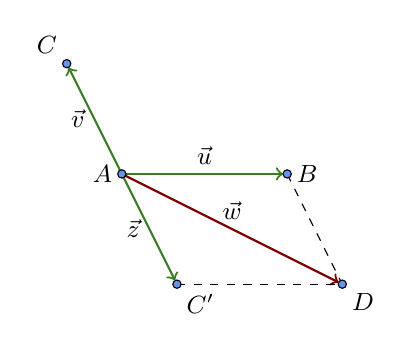
\begin{tikzpicture}[x=7mm,y=7mm, font=\small]

 \begin{scope}[thick, shorten >=1.5pt, ->]
  
	\draw[OliveGreen] (0,0) -- (-1,2);
	\draw[OliveGreen] (0,0) -- (1,-2);
	\draw[OliveGreen] (0,0) -- (3,0);  
	\draw[Maroon] (0,0) -- (4,-2);
      \end{scope}
  
\begin{scope}[dashed]
\draw (3,0) -- (4,-2);
\draw (1,-2) -- (4,-2);
\end{scope}
\begin{scope}[fill=CornflowerBlue, draw=black]
\filldraw (0,0) circle (1.5pt) node[left] {$A$};
\filldraw (3,0) circle (1.5pt) node[right] {$B$};
\filldraw (4,-2) circle (1.5pt) node[below right] {$D$};
\filldraw (1,-2) circle (1.5pt) node[below right] {$C'$};
\filldraw (-1,2) circle (1.5pt) node[above left] {$C$};
\end{scope}

\node[above] at (1.5,0) {$\vec{u}$};
\node[above] at (2,-1) {$\vec{w}$};
\node[left] at (.5,-1) {$\vec{z}$};
\node[left] at (-.5,1) {$\vec{v}$};
\end{tikzpicture}
 \caption{Differenza di due vettori.}
 \label{fig:F.11}
\end{figure}

\begin{exrig}
\begin{esempio}

Sono assegnati i vettori~$\vec{u}(4;0)$ e~$\vec{v}(-2;-1)$. Determinare~$\vec{d_1}=\vec{u}-\vec{v}$ e~$\vec{d_2}=\vec{v}-\vec{u}$. Cosa osservate?
\begin{center}
 % (c) 2012 Dimitrios Vrettos - d.vrettos@gmail.com

\begin{tikzpicture}[x=10mm,y=10mm, font=\small]

  \begin{scope}[->]
    \draw (-6.5,0) -- (6.5,0) node [below right] {$x$};
    \draw (0,-1.5) -- (0,1.5) node[above left] {$y$};
  \end{scope}

  \foreach \x/\xtext in {-6/-6,-5/-5,-4/-4,-3/-3,-2/-2,-1/-1,1/1,2/2,3/3,4/4,5/5,6/6}{
    \node[below] at (\x,0) {$\xtext$};
    \draw (\x,1.5pt) -- (\x,-1.5pt);}
  \foreach \y/\ytext in {-1/-1, 1/1}{
    \node[left] at (0,\y) {$\ytext$};
    \draw (1.5pt,\y) -- (-1.5pt,\y);}
  \node[below left] at (0,0) {$0$};

  \begin{scope}[dotted, orange]
    \draw (-6.5,-1.5) grid (6.5,1.5);
  \end{scope}

  \begin{scope}[thick, ->,shorten >=1.5pt]
    \draw[Maroon] (0,0) -- (4,0);  
    \draw[OliveGreen](0,0) -- (-2,-1);
  \end{scope}

  \begin{scope}[fill=CornflowerBlue, draw=black]
    \filldraw (0,0) circle (1.5pt)node [above left]{$O$};
    \filldraw (4,0) circle (1.5pt)node [above right]{$A$};
    \filldraw (-2,-1) circle (1.5pt) node [below left]{$C$};
  \end{scope}
  
  \node[above] at (2,0) {$\vec{u}$};
  \node[below] at (-1,-.5) {$\vec{v}$};

\end{tikzpicture}
\end{center}
\end{esempio}
\end{exrig}

\subsection{Moltiplicazione di un numero reale per un vettore}

\begin{definizione}
Assegnato un numero reale~$r$ ed un vettore~$\vec{v}$, il \emph{prodotto}
\[\vec{p} = r \cdot \vec{v}\]
è un vettore avente:
\begin{enumeratea}
\item la stessa direzione del vettore~$\vec{v}$;
\item intensità o modulo uguale al prodotto del modulo di~$\vec{v}$ per il valore assoluto di~$r$:
 \subitem $|\vec{p}|=|r| \cdot|\vec{v}|$;
\item verso uguale al verso di~$\vec{v}$ se~$r$ è positivo, verso opposto a quello di~$\vec{v}$ se~$r$ è negativo.
\end{enumeratea}
\end{definizione}

\begin{exrig}
\begin{esempio}
Nella figura sono rappresentati il vettore~$\vec{v}$ e altri vettori ottenuti moltiplicandolo per un numero reale:
$\vec{a}=2 \cdot \vec{v}$,~~$\vec{b}=-\dfrac{3}{2} \cdot \vec{v}$,~~$\vec{c}=\dfrac{1}{3} \cdot \vec{v}$.
\begin{center}
 % (c) 2012 Dimitrios Vrettos - d.vrettos@gmail.com

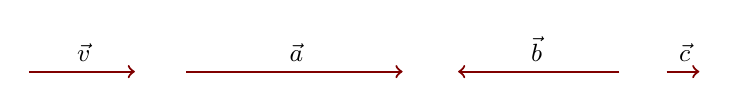
\begin{tikzpicture}[x=7mm,y=7mm, font=\small]

 \begin{scope}[thick, shorten >=1.5pt, ->, Maroon]
	\draw (0,0) -- (2,0); %vettore v
\node[above, black] at (1,0) {$\vec{v}$};
	\begin{scope}[xshift=20mm]
	\draw (0,0) -- (4,0); %vettore a
\node[above, black] at (2,0) {$\vec{a}$};
	\end{scope}
	\begin{scope}[xshift=54mm]
	\draw (3,0) -- (0,0); %vettore b
\node[above, black] at (1.5,0) {$\vec{b}$};
	\end{scope}
	\begin{scope}[xshift=81mm]
	\draw (0,0) -- (.67,0); %vettore c
\node[above, black] at (.33,0) {$\vec{c}$};
	\end{scope}
\end{scope}

\end{tikzpicture}
\end{center}

\end{esempio}
\begin{esempio}
Nel piano dotato di riferimento cartesiano ortogonale rappresentiamo il vettore~$\vec{u}(4;1)$; le componenti
del vettore~$\vec{p}=-2\cdot \vec{u}$ si ottengono moltiplicando per~$-2$ le componenti del vettore dato:~$\vec{p}(-8;-2)$. $\vec{p}$ e~$\vec{u}$
hanno la stessa direzione essendo~$m_{\vec{u}}=\frac{1}{4}=m_{\vec{p}}$ e anzi appartengono alla stessa retta avendo in comune il punto di applicazione $O(0;0)$.
\begin{center}
 % (c) 2012 Dimitrios Vrettos - d.vrettos@gmail.com

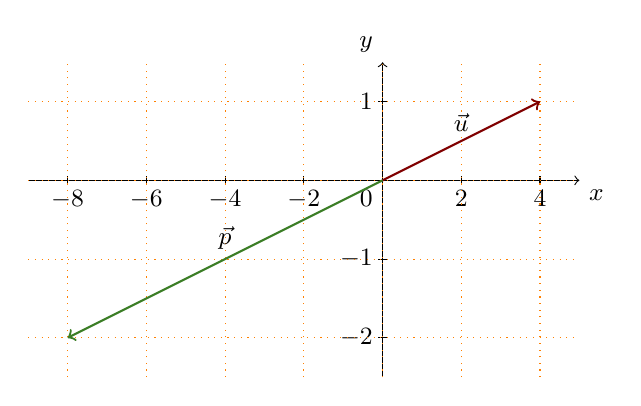
\begin{tikzpicture}[x=10mm,y=10mm, font=\small]

  \begin{scope}[->]
    \draw (-4.5,0) -- (2.5,0) node [below right] () {$x$};
    \draw (0,-2.5) -- (0,1.5) node[above left] {$y$};
  \end{scope}

  \foreach \x/\xtext in {-4/-8, -3/-6,-2/-4,-1/-2,1/2,2/4}{
    \node[below] at (\x,0) {$\xtext$};
    \draw (\x,1.5pt) -- (\x,-1.5pt);}
  \foreach \y/\ytext in {-2/-2,-1/-1, 1/1}{
    \node[left] at (0,\y) {$\ytext$};
    \draw (1.5pt,\y) -- (-1.5pt,\y);}
  \node[below left] at (0,0) {$0$};

  \begin{scope}[dotted, orange]
    \draw (-4.5,-2.5) grid (2.5,1.5);
  \end{scope}

  \begin{scope}[thick, ->]
	\draw[Maroon] (0,0) -- (2,1);  
	\draw[OliveGreen](0,0) -- (-4,-2);
      \end{scope}
 
\node[above] at (1,.5) {$\vec{u}$};
\node[above] at (-2,-1) {$\vec{p}$};
\end{tikzpicture}
\end{center}
\end{esempio}
\end{exrig}

In generale, dato un vettore~$\vec{u}(x_u;y_u)$ si ha che~$r \cdot \vec{u} = \vec{p}(r \cdot x_u; r \cdot y_u)$, quindi la sua direzione è $m_{\vec{p}}=\frac{r \cdot y_u}{r \cdot x_u}=\frac{y_u}{x_u}= m_{\vec{u}}$, cioè la stessa di $\vec{u}$.

\begin{osservazione}
Se due vettori hanno la stessa direzione, cioè appartengono a rette parallele, si può sempre trovare un numero reale~$r$
tale che uno sia~$r$ volte l'altro. La figura seguente può suggerirvi come giustificare l'osservazione precedente.
\begin{center}
 % (c) 2012 Dimitrios Vrettos - d.vrettos@gmail.com

\begin{tikzpicture}[x=10mm,y=10mm, font=\small]

  \begin{scope}[->, thick]
\draw[OliveGreen] (0,0) -- (4,0);
\draw[Maroon] (1,1) -- (3,1);
\end{scope}
\node[above] at (2,1) {$\vec{u}$};
\node[above] at (2,0) {$\vec{v}$};
\begin{scope}[dotted]
\draw (0,0) -- (2,2)--(4,0);
\end{scope}
\end{tikzpicture}
\end{center}
\end{osservazione}

\begin{exrig}
\begin{esempio}

Sono assegnati i vettori~$\vec{x}(\frac {1}{2};1)$, $\vec{y}(-3;-1)$ e $\vec{z}(0;3)$.
Costruite i vettori~$\vec{p_1}=2 \cdot \vec{x}-\vec{y}$,~~$\vec{p_2}=2 \cdot (\vec{z}+\vec{y})$,~~$\vec{p_3}=-\frac {3}{2} \cdot \vec{z} +2 \cdot \vec{y}+3 \cdot \vec{x}$
e determinatene le componenti.
\end{esempio}
\end{exrig}


\ovalbox{\risolvii \ref{ese:B.4}, \ref{ese:B.5}, \ref{ese:B.6}}

\section{Dipendenza e indipendenza lineare}

\begin{definizione}
Diciamo che un vettore~$\vec{v}$ è \emph{combinazione lineare} di altri vettori~$\vec{x}$, $\vec{y}$, $\vec{z}$ se esistono
i numeri reali~$r_1$, $r_2$, $r_3$, detti \emph{coefficienti della combinazione lineare}, per i quali risulta verificata
l'uguaglianza~$\vec{v}=r_1 \cdot \vec{x} + r_2 \cdot \vec{y} + r_3 \cdot \vec{z}$.
\end{definizione}
%\newpage
\begin{exrig}
\begin{esempio}
Nell'esempio precedente hai costruito i vettori~$\vec{p_1}$, $\vec{p_2}$, $\vec{p_3}$ eseguendo la somma algebrica di vettori costruiti moltiplicando
per numeri reali i vettori assegnati~$\vec{x}$, $\vec{y}$, $\vec{z}$. Possiamo dire che:
\begin{itemize*}
\item $\vec{p_1}$ è combinazione lineare dei vettori~$\vec{x}$ e~$\vec{y}$ i cui coefficienti sono~$r_1=2$, $r_2=-1$.
\item $\vec{p_2}$ è combinazione lineare dei vettori~$\vec{z}$ e~$\vec{y}$ i cui coefficienti sono~$r_1=2$, $r_2=2$.
\item $\vec{p_3}$ è combinazione lineare dei vettori~$\vec{x}$, $\vec{y}$ e~$\vec{z}$ i cui coefficienti sono~$r_1=-\frac{3}{2}$, $r_2=2$ e $r_3=3$.
\end{itemize*}
\end{esempio}
\end{exrig}

Nell'insieme~$\spV$ di tutti i vettori del piano cartesiano, consideriamo i vettori~$\vec{i}(1;0)$ e~$\vec{j}(0;1)$ appartenenti
rispettivamente all'asse delle ascisse e a quello delle ordinate; possiamo notare che $\vec{i}$ e $\vec{j}$ formano tra loro un angolo di $90\grado$ e che $|\vec{i}|=|\vec{j}|=1$. Tali vettori sono chiamati \emph{versori} associati rispettivamente dell'asse $x$ e all'asse $y$.

Ogni vettore~$\vec{v}$ del piano può essere scritto come combinazione lineare di~$\vec{i}$ e~$\vec{j}$ e le sue componenti sono i coefficienti
della combinazione lineare di $\vec{i}$ e $\vec{j}$ con i quali si determina~$\vec{v}$.
\[\vec{v}(x_v;y_v)=x_v \cdot \vec{i}+y_v \cdot \vec{j}\]

\ovalbox{\risolvi \ref{ese:B.7}}

\begin{exrig}
\begin{esempio}
Disegniamo nel riferimento cartesiano ortogonale i vettori~$\vec{u}(1;1)$, $\vec{v}(4;-2)$, $\vec{w}(3;1)$; ci chiediamo se è possibile scrivere~$\vec{w}$
come combinazione lineare degli altri due.
\begin{center}
 % (c) 2012 Dimitrios Vrettos - d.vrettos@gmail.com

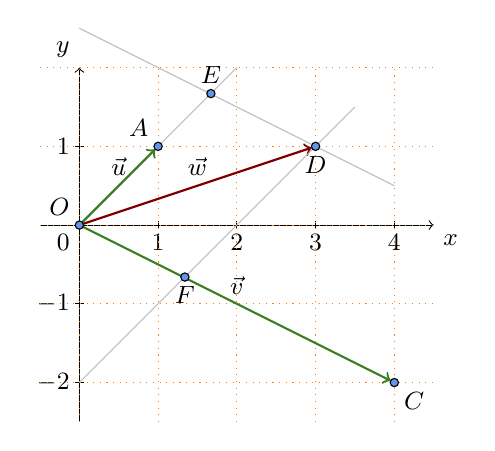
\begin{tikzpicture}[x=10mm,y=10mm, font=\small]

  \begin{scope}[->]
    \draw (-.5,0) -- (4.5,0) node [below right] {$x$};
    \draw (0,-2.5) -- (0,2) node[above left] {$y$};
  \end{scope}

  \foreach \x/\xtext in {1/1,2/2,3/3,4/4}{
    \node[below] at (\x,0) {$\xtext$};
    \draw (\x,1.5pt) -- (\x,-1.5pt);}
  \foreach \y/\ytext in {-2/-2,-1/-1, 1/1}{
    \node[left] at (0,\y) {$\ytext$};
    \draw (1.5pt,\y) -- (-1.5pt,\y);}
  \node[below left] at (0,0) {$0$};

  \begin{scope}[dotted, orange]
    \draw (-.5,-2.5) grid (4.5,2);
  \end{scope}

  \begin{scope}[thick, ->,shorten >=1.5pt]
	\draw[Maroon] (0,0) -- (3,1);     % OD
	\draw[OliveGreen](0,0) -- (1,1);  % OA
	\draw[OliveGreen](0,0) -- (4,-2); % OC
      \end{scope}
 
\begin{scope}[lightgray]
\draw (1,1) -- (2,2);
\draw[xshift=20mm] (-2,-2) -- (1.5,1.5);
\draw[yshift=25mm](0,0)--(4,-2);
\end{scope}

\begin{scope}[fill=CornflowerBlue, draw=black]
\filldraw (0,0) circle (1.5pt)node [above left]{$O$};
\filldraw (3,1) circle (1.5pt)node [below]{$D$};
\filldraw (1,1) circle (1.5pt)node [above left]{$A$};
\filldraw (1.34,-.66) circle (1.5pt)node [below]{$F$};
\filldraw (1.67,1.67) circle (1.5pt) node [above]{$E$};
\filldraw (4,-2) circle (1.5pt) node [below right]{$C$};
\end{scope}

\node[above] at (0.5,0.5) {$\vec{u}$};
\node[above] at (2,-1) {$\vec{v}$};
\node[above] at (1.5,0.5) {$\vec{w}$};

\end{tikzpicture}
\end{center}


\paragraph{Il metodo geometrico} Dobbiamo costruire due vettori~$\vec{u}'=r_1 \cdot \vec{u}$ e~$\vec{v}'=r_2 \cdot \vec{v}$ tali che sommati diano
il vettore~$\vec{w}$. Dal punto~$D$ tracciamo la parallela alla retta~$OC$, che interseca la retta~$AO$ nel punto~$E$; dallo stesso punto~$D$
tracciamo la parallela alla retta~$AO$ che interseca in~$F$ la retta~$OC$. I punti~$E$ ed~$F$ sono gli
estremi dei due vettori~$\vec{u}'$ e $\vec{v}'$ cercati: $\vec{u}'=\overrightarrow{OE}=r_1 \cdot \vec{u}$ e~$\vec{v}'=\overrightarrow{OF}=r_2 \cdot \vec{v}$ con~$r_1>1$ e~$r_2<1$ rispettivamente ottenuti
allungando e accorciando~$\vec{u}$ e~$\vec{v}$. Si ha quindi~$\vec{w}=r_1 \cdot \vec{u} + r_2 \cdot \vec{v}$.

\paragraph{Il metodo algebrico} Dobbiamo trovare due numeri~$r_1$ e~$r_2$ tali che
\[ \vec{w}=r_1 \cdot \vec{u}+r_2 \cdot \vec{v} \quad\Rightarrow\quad
\left\{\begin{array}{l}
3=1 \cdot r_1+1 \cdot r_2 \quad\text{(componenti }x\text{)} \\
1=1 \cdot r_1-2 \cdot r_2 \quad\text{(componenti }y\text{)}
\end{array}\right. \]
%\newpage
e risolvendo il sistema lineare di due equazioni in due incognite si ottiene~$r_1=\frac{5}{3}$ e~$r_2=\frac{1}{3}$, coerentemente ai risultati della costruzione geometrica effettuata.
\end{esempio}
\end{exrig}

\ovalbox{\risolvi \ref{ese:B.8}}

\begin{definizione}
Dati $n$ vettori $\vec{v}_1$, $\vec{v}_2$, \ldots, $\vec{v}_n$, questi si dicono \emph{linearmente indipendenti} se almeno uno di essi si può scrivere come combinazione lineare degli altri. Se nessuno degli $n$ vettori $\vec{v}_1$, $\vec{v}_2$, \ldots, $\vec{v}_n$ può essere scritto come combinazione lineare degli altri, i vettori si dicono \emph{linearmente indipendenti}.
\end{definizione}

\vspazio\ovalbox{\risolvii \ref{ese:B.9}, \ref{ese:B.10}}

\newpage
% (c) 2012 Silvia Cibola - silvia.cibola@gmail.com
% (c) 2012 - 2014 Dimitrios Vrettos - d.vrettos@gmail.com

\section{Esercizi}

\subsection{Esercizi dei singoli capitoli}

\subsubsection*{B.1 - Prime definizioni}
\begin{esercizio}
\label{ese:B.1}
Segnate nel piano dotato di riferimento cartesiano ortogonale i vettori~$\vec{v}(1;2)$ e~$\vec{w}(3;-1)$. Possiamo affermare che~$|\vec{w}|=2 \cdot |\vec{v}|$?
\end{esercizio}

\subsubsection*{B.2 - Operazioni con i vettori}
\begin{esercizio}
\label{ese:B.2}
Provate a giustificare la seguente affermazione: l'operazione di addizione definita secondo la regola del parallelogramma gode della proprietà commutativa.
\end{esercizio}

\begin{esercizio}
\label{ese:B.3}
Determinate il vettore~$\vec{z}=\vec{u}+\vec{w}$ essendo~$\vec{u}(-1;-3)$ e~$\vec{v}(2;-1)$. Determinate inoltre il modulo di~$\vec{z}$ e la sua direzione.
Potete affermare che~$|\vec{z}|=|\vec{u}|+|\vec{w}|$?
\end{esercizio}

\begin{esercizio}
\label{ese:B.4}
Nel riferimento cartesiano ortogonale riportato di seguito sono rappresentati i vettori~$\vec{u}$ e~$\vec{v}$. Completate:

\begin{enumeratea}
\item il vettore~$\vec{u}$ è applicato all'origine e ha componenti~$\ldots$;
\item il vettore~$\vec{v}$ ha il primo estremo in~$B(\ldots;\ldots)$ e il secondo in~$\ldots$, pertanto le sue componenti sono~$\ldots$;
\item $m_{\vec{u}}=\ldots$ e~$m_{\vec{v}}=\ldots$, pertanto essi sono~$\ldots$;
\item $|\vec{u}|=\ldots$ e~$|\vec{v}|=\ldots$;
\item determinare~$r$ in modo che~$\vec{v}=r \cdot \vec{u}$.
\end{enumeratea}
\begin{center}
 % (c) 2012 Dimitrios Vrettos - d.vrettos@gmail.com

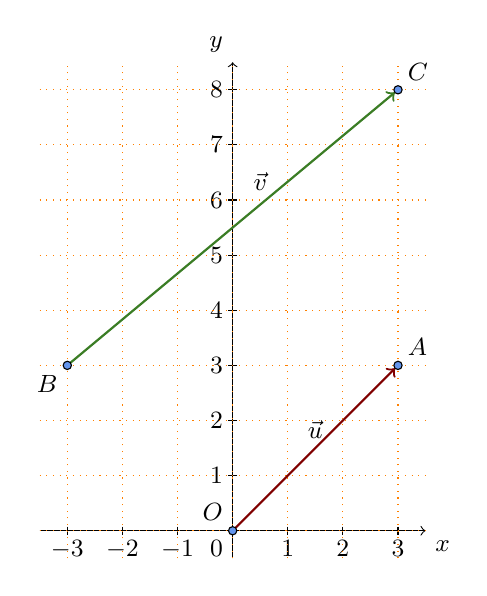
\begin{tikzpicture}[x=7mm,y=7mm, font=\small]

  \begin{scope}[->]
    \draw (-3.5,0) -- (3.5,0) node [below right] {$x$};
    \draw (0,-.5) -- (0,8.5) node[above left] {$y$};
  \end{scope}

  \foreach \x/\xtext in {-3/-3,-2/-2,-1/-1,1/1,2/2,3/3}{
    \node[below] at (\x,0) {$\xtext$};
    \draw (\x,1.5pt) -- (\x,-1.5pt);}
  \foreach \y/\ytext in {1/1,2/2,3/3,4/4,5/5,6/6,7/7,8/8}{
    \node[left] at (0,\y) {$\ytext$};
    \draw (1.5pt,\y) -- (-1.5pt,\y);}
  \node[below left] at (0,0) {$0$};

  \begin{scope}[dotted, orange, step=7mm]
    \draw (-3.5,-.5) grid (3.5,8.5);
  \end{scope}

  \begin{scope}[thick, ->,shorten >=1.5pt]
	\draw[Maroon] (0,0) -- (3,3);  
	\draw[OliveGreen](-3,3) -- (3,8);
      \end{scope}
 

\begin{scope}[fill=CornflowerBlue, draw=black]
\filldraw (0,0) circle (1.5pt)node [above left]{$O$};
\filldraw (3,3) circle (1.5pt)node [above right]{$A$};
\filldraw (-3,3) circle (1.5pt)node [below left]{$B$};
\filldraw (3,8) circle (1.5pt) node [above right]{$C$};
\end{scope}
\node[above] at (1.5,1.5) {$\vec{u}$};
\node[above] at (.5,6) {$\vec{v}$};
\end{tikzpicture}
\end{center}

\end{esercizio}

\begin{esercizio}
\label{ese:B.5}
Determinate le componenti del vettore~$\vec{w}=2 \cdot \vec{v}$ essendo~$\vec{v}(\frac{3}{2};-2)$. Verificate che~$\vec{w}$ e~$\vec{v}$ hanno stessa direzione
e~$|\vec{w}|=2 \cdot |\vec{v}|$.
\end{esercizio}

\begin{esercizio}
\label{ese:B.6}
Verificate che~$\frac{3}{2} \cdot (\vec{x}+\vec{y})=\frac{3}{2}\vec{x}+\frac{3}{2}\vec{y}$ essendo~$\vec{x}(-\frac{5}{4};1)$ e~$\vec{y}(4;-1)$.
\end{esercizio}
\pagebreak
\subsubsection*{B.3 - Dipendenza e indipendenza lineare}
\begin{esercizio}
\label{ese:B.7}
Completate le scritture:
\begin{multicols}{2}
\begin{enumeratea}
\item $\vec{v}(-\sqrt{2};\frac {5}{4})=\ldots \cdot \vec{i}+\ldots \cdot \vec{j}$;
\item $\vec{u}(1;-1)=\ldots \cdot \vec{i}+\ldots \cdot \vec{j}$;
\item $\vec{h}(\ldots;\ldots)=\frac {\sqrt{3}}{3} \cdot \vec{i}-9 \cdot \vec{j}$;
\item $\vec{z}(\ldots;\ldots)=\frac {3 \sqrt{5}}{3} \cdot \vec{i}$;
\end{enumeratea}
\end{multicols}
\end{esercizio}

\begin{esercizio}
\label{ese:B.8}
\begin{multicols}{2}
 Dati i vettori della figura a fianco, applicate il metodo geometrico per determinare i vettori che permettono di scrivere~$\vec{w}$ come combinazione lineare degli altri due.
Riprendete questi stessi vettori e determinate i vettori che permettono di scrivere~$\vec{v}$ come combinazione lineare degli altri due. In maniera analoga, determinate i vettori che permettono di scrivere~$\vec{u}$ come combinazione lineare degli altri due ($\vec{v}$ e $\vec{w}$).
\begin{center}
% (c) 2012 Dimitrios Vrettos - d.vrettos@gmail.com

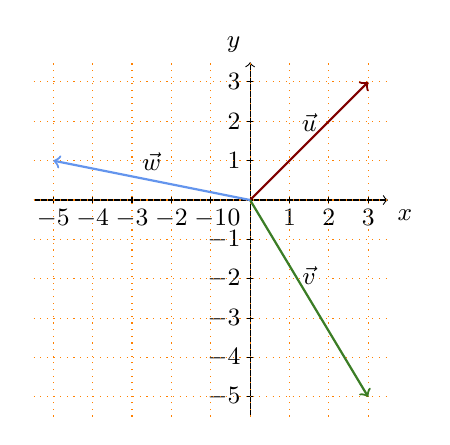
\begin{tikzpicture}[x=5mm,y=5mm, font=\small]

  \begin{scope}[->]
    \draw (-5.5,0) -- (3.5,0) node [below right] {$x$};
    \draw (0,-5.5) -- (0,3.5) node[above left] {$y$};
  \end{scope}

  \foreach \x/\xtext in {-5/-5,-4/-4,-3/-3,-2/-2,-1/-1,1/1,2/2,3/3}{
    \node[below] at (\x,0) {$\xtext$};
    \draw (\x,1.5pt) -- (\x,-1.5pt);}
  \foreach \y/\ytext in {-5/-5,-4/-4,-3/-3,-2/-2,-1/-1,1/1,2/2,3/3}{
    \node[left] at (0,\y) {$\ytext$};
    \draw (1.5pt,\y) -- (-1.5pt,\y);}
  \node[below left] at (0,0) {$0$};

  \begin{scope}[dotted, orange, step=5mm]
    \draw (-5.5,-5.5) grid (3.5,3.5);
  \end{scope}

  \begin{scope}[thick, ->]
	\draw[Maroon] (0,0) -- (3,3);  
	\draw[OliveGreen](0,0) -- (3,-5);
	\draw[CornflowerBlue] (0,0) -- (-5,1);
      \end{scope}
 
\node[above] at (1.5,1.5) {$\vec{u}$};
\node[above] at (1.5,-2.4) {$\vec{v}$};
\node[above] at (-2.5,.5) {$\vec{w}$};
\end{tikzpicture}
\end{center}
\end{multicols}
\end{esercizio}

\begin{esercizio}
\label{ese:B.9}
I vettori dell'esercizio precedente sono linearmente dipendenti?
\end{esercizio}

\begin{esercizio}
\label{ese:B.10}
Spiegate perché i tre vettori~$\vec{v}(1;2)$, $\vec{u}(3;1)$ e~$\vec{w}(-3;-6)$ sono linearmente dipendenti.
\end{esercizio}


\cleardoublepage
